
\begin{question}
Please make a frequency table and a frequency histogram from the
following (unsorted) continuous data by rounding to the nearest integer.

\begin{longtable}[]{@{}rrrrrr@{}}
\toprule
\endhead
34.2282 & 33.4619 & 35.0504 & 36.5544 & 34.6125 & 32.7785\tabularnewline
35.2745 & 34.7295 & 35.8640 & 33.1210 & 34.7377 & 35.5176\tabularnewline
34.5648 & 33.8892 & 33.7858 & 33.4916 & 36.8922 & 33.6199\tabularnewline
37.3664 & 36.3487 & 36.5729 & 34.6641 & 33.0986 & 37.0611\tabularnewline
36.1932 & 35.8686 & 32.6269 & 37.3401 & 35.8037 & 32.3844\tabularnewline
\bottomrule
\end{longtable}
\end{question}

\begin{solution}
Make a frequency table.

\begin{longtable}[]{@{}rr@{}}
\toprule
bin & frequency\tabularnewline
\midrule
\endhead
32 & 1\tabularnewline
33 & 6\tabularnewline
34 & 4\tabularnewline
35 & 7\tabularnewline
36 & 6\tabularnewline
37 & 6\tabularnewline
\bottomrule
\end{longtable}

Make the histogram.

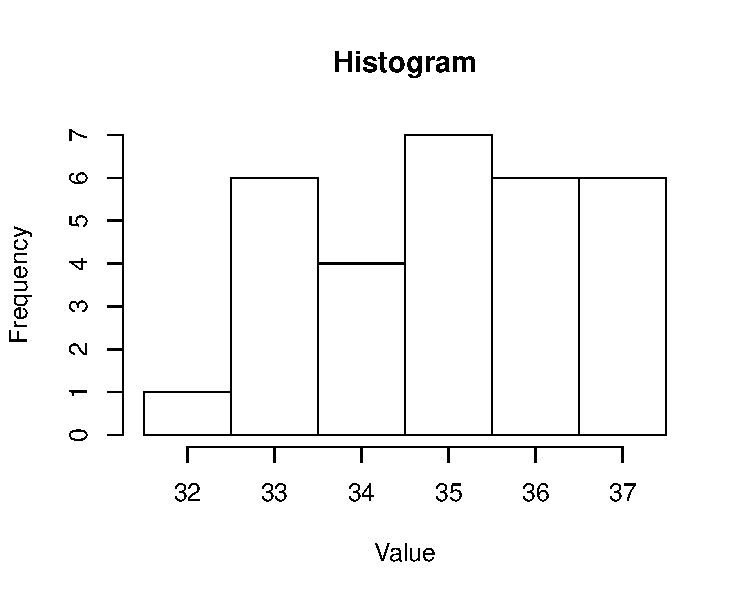
\includegraphics{barchart-1-4.pdf}\\
\end{solution}

